\section{Era uma vez uma enciclopédia colaborativa}

A origem da Wikipédia e a tradição enciclopedista já foram contadas diversas vezes e de diferentes formas por vários pesquisadores, e neste trabalho não nos propomos a refazer estes esforços.\footnote{Ao leitor que desejar se aprofundar na origem do enciclopedismo, recomendamos a leitura do capítulo "O enciclopedismo de Plínio a Jimmy Wales, em (\cite{esteves_as_2014}).} Em nossa análise nos interessamos pelo movimento presente do fazer da Wikipédia que, segundo Jankowski (\citeyear{jankowski_wikipedia_2013}), é caraterizada pela colaboração, co-construção, cooperação, confiança na comunidade e construcionismo, em oposição à tradição enciclopedista, que se baseia nos valores epistêmicos de utilitarismo, organização sistêmica, autoridade, confiança em especialistas e consistência.

Esta diferenciação de valores pode ser vista como uma ruptura que se sustenta a partir da ``\textit{produção colaborativa feita por editores voluntários. Não há um projeto norteando seu desenvolvimento. Os artigos são criados e dimensionados conforme o desígnio dos colaboradores (...). Ela parece romper, portanto, com o modelo de produção de conteúdo confiada a especialistas, predominante no enciclopedismo pelo menos desde a Encyclopédie}''  \citep[p.61]{esteves_as_2014}. Segundo Demo (\citeyear{demo_conhecimento_2009}), essa ``\textit{conclamação à sociedade em geral para produzir conhecimento}'' é algo nunca antes visto, pois ``\textit{produzir conhecimento sempre foi atividade reservada, preservada, censurada (Shattuck, 1996. Rescher, 1987), tendo como patrulheiros os especialistas e as entidades que os abrigavam.}'' \citep{demo_conhecimento_2009}.

A conclamação apresenta resultados visíveis em números: hoje, a auto-intitulada ``\textit{enciclopédia livre, que qualquer um pode editar}'' é o décimo site mais visitado do mundo \citep{alexa_2019}, contando com enciclopédias em 303 idiomas diferentes. Cabe destacar que, ainda que traduções sejam permitidas, cada enciclopédia tem sua escrita feita de forma independente  \citewiki{ptwiki_sobre} com políticas editoriais e regras de convivência que podem variar de acordo com as comunidades locais. \citep{marques_wikipedia_2013}. Ao final de 2019, suas 303 versões diferentes somadas apresentavam cifras impressionantes: mais de 40 milhões de verbetes, 400 mil editores ativos por mês e 500 milhões de visitantes únicos também por mês. \citep{wikimedia_stats_2019}

Em meio a tantos verbetes, visitantes e editores, é interessante notar a dificuldade da Wikipédia em se definir. Buscando sua identidade, a comunidade prefere usar a negação do que a afirmação. Em momentos de ruptura e conflito, aparenta ser mais fácil falar o que não se é do que o que se é. Tal movimento não é novidade, e pode ser encontrado por exemplo na fala de Tião Rocha, relatada em Severo (\citeyear[p. 19-20]{severo_tics_2016}): ``\textit{Tião tirou do chapéu-cartola a seguinte matreirice: \textbf{os não-objetivos} da educação. Ele escreveu um documento, similar a um manifesto, onde estava \textbf{listado tudo aquilo que aquele grupo não queria} que acontecesse com os filhos dos outros em uma escola (...) o nosso compromisso é: se nós não fizermos o que está listado nessa folha, o resto é lucro}''.\footnote{Grifos nossos.}

Tal qual uma pintura onde a figura é revelada a partir da construção do fundo, na página ``\textit{O que a Wikipédia não é}'' a comunidade lusófona pinta seus transbordamentos apresentando 20 seções textuais, cada uma dedicada a versar sobre algo que deve estar fora de seu enquadramento. Começando por não ser uma ``\textit{enciclopédia impressa}'', deixando claro no caminho ``\textit{não ser um consultório médico}'' nem ``\textit{um campo de batalha}'', e concluindo com a afirmação de que ``\textit{não é uma sociedade secreta}''. \citewiki{ptwiki_naoe}.

A construção de ``o que a Wikipédia não é'' mobiliza muito mais a comunidade do que dizer para o mundo afirmativamente o que ela é. A página “Sobre a Wikipédia”, primeiro link visto por um usuário que acesse a página principal da Wikipédia em português, tem um conteúdo bem mais tímido que sua contraparte negacionista,  contando com quatro seções que totalizam 5.889 bytes, desenvolvidos em 215 edições feitas por 134 editores distintos 
\footnote{Dados encontrados em https://xtools.wmflabs.org/articleinfo/pt.wikipedia.org/Wikipédia:Sobre\_a\_Wikipédia?uselang=pt-br , acessada em 11 de abril de 2020.}. Já a página sobre seus transbordamentos é mais que cinco vezes maior, com 33.503 bytes trabalhados em 412 edições por 149 diferentes editores. 
\footnote{Dados encontrados em https://xtools.wmflabs.org/articleinfo/pt.wikipedia.org/Wikipédia:O\_que\_a\_Wikipédia\_não\_é?uselang=pt-br , acessada em 11 de abril de 2020.} 

Pesquisar uma comunidade que tem dificuldades em dizer o que é tráz claramente dificuldades e desafios. Em nossos esforços de realizar análises quantitativas coladas aos bancos de dados, precisamos criar recortes e métricas que, ao descrever o que está sendo estudado, também o prescreve e, portanto, nossas escolhas podem apontar para definições do que ``a Wikipédia é'' que não sejam consensuais.

Apresentando um exemplo concreto, trabalhamos na pesquisa com recortes de usuários tanto por grupos de tipo de permissão de acesso ao MediaWiki como por atividades em diferentes espaços da enciclopédia. A relevância tanto dos estatutos \footnote{Estatuto é como a comunidade se refere às permissões que um usuário ganha ao fazer parte de um grupo de usuários no MediaWiki.} como dos espaços de participação escolhidos como representativos pela pesquisa desta dissertação pode ser reafirmada ou deslegitimada, a depender do que se entenda afinal ser a Wikipédia e suas comunidades.

O termo ``comunidades'' aliás é muito utilizado no mundo da Wikipédia e sua abrangência varia bastante de acordo com o escopo tratado. Por exemplo, a ``comunidade de wikipedistas'' engloba todos os atores pelo mundo que atuam em alguma Wikipédia. Já o termo ``comunidade lusófona'' irá se referir apenas aos que participam da Wikipédia em português. Assim, cada projeto\footnote{Projeto" é a forma como as comunidades se referenciam a cada instância wiki distinta.} tem sua comunidade que é a autora de seus conteúdos e gestora de sua governança, dentro dos limites permitidos pelo Movimento Wikimedia.\footnote{O Movimento Wikimedia nasceu da expansão da Wikipédia, que em busca de realizar seu objetivo principal enunciado como ``Imagine um mundo onde cada pessoa do planeta tenha acesso livre a soma de todo conhecimento da humanidade. É isso que estamos fazendo'' decidiu ao longo do tempo criar outros projetos de construção coletiva de conhecimento para abarcar conteúdos que segundo as políticas editoriais não seriam considerados enciclopédicos. Assim nascem Wikcionário, Wikilivros, Wikinotícias, Wikivoyage e diversas outras wikis com suas próprias comunidades, não necessariamente interessadas na construção enciclopédias. Assim, o Movimento Wikimedia passa a ser entendido como a união das comunidades de todos esses projetos (e também das comunidades de desenvolvedores de softwares de/para wikis, que detalharemos posteriormente) e cabe a ele, através da Fundação Wikimedia, definir regras gerais que devem ser seguidas por todos os projetos.}

A compreensão do que é ou não uma Wikipédia varia ao longo de suas diversas comunidades, e pode encontrar consensos locais que não sejam globais. A própria página “O que não é a Wikipédia”, se observada em outros idiomas, terá algumas seções em comum e outras divergentes. Enquanto a versão em português conta com 20 tópicos, suas correlatas apresentam 19 tópicos em inglês, 22 em francês, 14 em espanhol e 9 itens em alemão.\footnote{ \citewiki{enwiki_isnot}; \citewiki{frwiki_nest}; \citewiki{eswiki_noes}; \citewiki{dewiki_nichtist}}. 

Não avançamos na diferença entre os conteúdos destas páginas pois em nossa pesquisa preferimos trabalhar com as definições que se constituem na prática cotidiana das comunidades. Observamos então a configuração das comunidades ditada a partir da prática wikipédica de produção coletiva de conteúdos, seguindo suas dinâmicas e especificidades.

\subsection{A escrita wikipédica}

Inspirada abertamente pelo movimento software livre desde sua fundação \citep{lih_wikirevolution_2009}, a Wikipédia se distancia da prática de escrita tradicional enciclopédica ao ter sua política editorial centrada em escritores não-especialistas e em coautoria massiva. Tomando emprestado o termo de Tião Rocha apud (\cite{severo_tics_2016}), esse ``\textit{empodimento}''\footnote{Versão localizada do termo em inglês \textit{empowerment}} é uma característica que distancia o fazer da Wikipédia da prática de escrita científica, tradicionalmente exercida por um autor solitário, o especialista, ou com poucos coautores.

Ao estudar a prática de historiadores, Rosenzweig (\citeyear{rosenzweig_can_2006}) diz existir um individualismo possessivo na produção de conteúdos, e atenta para o fato de ser considerada uma boa prática na área sempre citar o nome do autor quando for se referir a uma ideia, mesmo que esteja sendo lateralmente mencionada e já seja consensual entre os interlocutores. Complementando que ``\textit{um trabalho de história sem donos, ou com múltiplos donos anônimos, é algo inimaginável em nossa prática profissional.}''\footnote{Tradução livre do original em inglês: ``A historical work without owners and with multiple, anonymous authors is thus almost unimaginable in our professional culture.''} 

Nesta mesma toada caminha a ciência como um todo em seus textos. Como nos ensina a também historiadora Juliana Marques, ``\textit{na academia supõe-se como condição sine qua non que haja um ou mais autores para determinado texto, responsáveis pelo conteúdo e que tenham uma qualificação mínima reconhecida por seus pares para que se justifique a autoridade de sua argumentação. São proprietários do texto na sua forma total, e a reapropriação, fragmentação e modificação deste sem prévia autorização constitui plágio, reconhecido legalmente como crime}''. \citep[337]{marques_trabalhando_2012}

A escrita coletiva feita por anônimos permite observar colaborações na construção de conteúdos de forma estável por certo tempo, e, assim como o fazer da ciência, a escrita da Wikipédia segue um ``\textit{caminho muito estranho porque é invisível quando tudo vai bem}'' \citep[p.44]{latour_cogitamus_2010}. Porém, no contínuo exercício de escrita e revisão das edições feitas entre usuários, como seria de se esperar, divergências e controvérsias emergem, quebrando o moto contínuo de estabilidade editorial e demandando desvios, que ensejam novas abordagens, formas de agir, regras e ferramentas tecnológicas. São estes casos, onde acontecem enredamentos de diferentes elementos em busca de novas estabilizações, que exploraremos para entender o funcionamento prático da enciclopédia.

Um dos movimentos mais exemplares deste enredamento de novos elementos para estabilização de controvérsias é a busca por aliados que sustentem um determinado texto. Curiosamente, apesar das diferenças entre as práticas de escrita wikipédica e científica apontadas acima, a busca por aliados mais poderosos para reforçar uma posição é tão similar em ambos processos de escrita que a seguinte passagem de Latour (\citeyear[p.48]{latour_cogitamus_2010}), originalmente sobre textos científicos, poderia muito bem versar sobre a Wikipédia: ``\textit{A presença ou ausência de referências, citações e notas de rodapé é um sinal tão importante de que o documento é ou não sério que um fato pode ser transformado em ficção ou uma ficção em fato apenas com o acréscimo ou a subtração de referências}''.

Esta dança literária, praticada por editores e textos em busca de um lugar ao sol na maior enciclopédia do mundo, acontece em páginas públicas, onde todas as mensagens, controvérsias e históricos de alteração estão acessíveis a qualquer leitor. Porém, o fato de estar lá disponível não significa que na prática a grande maioria dos leitores acesse estes espaços.

No mesmo movimento da ciência que exibe uma face pronta e outra ainda em construção, ilustrado por Latour (\citeyear{latour_ciencia_1987}) através duas faces de Jano bifronte, a Wikipédia também tem suas duas faces distintas. Enquanto uma, conhecida do grande público, apresenta textos grandes, ilustrados e referenciados, a outra é incerta, instável, está em constante movimento para ganhar uma forma estável e é conhecida por poucos.

\begin{figure}[H]
    \centering
    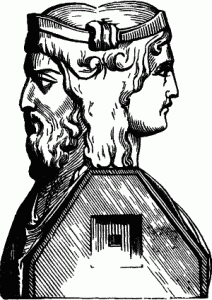
\includegraphics[width=0.5\textwidth]{Images/duas_faces_jano.png}
    \caption{As duas faces de Jano bifronte.}
    \label{fig:duas_faces_jano}
\end{figure}

É esta segunda face, sempre em construção e distante das vistas da grande audiência, que expressa a criação das regras e dinâmicas que interessam à investigação proposta neste capítulo. Seguindo os traços deste rosto encontramos acirradas disputas sobre qualidade editorial, grupos de usuários atuando em funções administrativas, robôs e demais elementos que serão explorados nas seções a seguir.

\subsection{Busca por qualidade}

Enquanto milhões de pessoas acessam diariamente a maior enciclopédia do mundo, uma rede de elementos heterogêneos está 24 horas se movimentando para garantir a estabilidade do que é apresentado. Uma rede de atores humanos e não-humanos (usuários, robôs, fundações, filtros, referências, métricas, ferramentas, políticas editoriais ...) faz o trabalho pesado semi invisível para que a maioria dos leitores desinteressados possam apenas enxergar textos e figuras estabilizados.

Em meio a essa incessante busca por garantir a qualidade dos conteúdos apresentados, no processo de proteger a enciclopédia de edições danosas é recorrente que usuários novatos, ainda não familiarizados com as políticas editoriais da enciclopédia, sejam tratados como vândalos\footnote{O termo ``vandalismo'' neste contexto se refere a edições de má fé feitas na Wikipédia.} \citep{halfaker_snuggle:_2014}. Este problema é habitual motivo de debates em vários espaços de discussão da Wikipédia, como o Projeto AntiVandalismo\footnote{Portal disponível em https://pt.wikipedia.org/wiki/Wikipédia:Projetos/AntiVandalismo .}, com usuários buscando estratégias para combater o vandalismo sem ``jogar fora o bebê junto com a água do banho''.

Na busca por formas de separar novatos bem-vindos na comunidade daqueles que se deseja afastar já foram propostas diversas iniciativas, desde mudanças comportamentais de editores patrulhadores à utilização de ferramentas automatizadas, que vão do uso de filtros de edições e captchas\footnote{Captcha, ``\textit{Completely Automated Public Turing test to tell Computers and Humans Apart}'', é uma funcionalidade presente em vários sistemas que intenta descobrir se o usuário é um humano ou um robô.} no MediaWiki a robôs que realizam reversões e enviam boas-vindas \citep{halfaker_bots_2012} e modelos de aprendizado de máquina (também chamados de inteligências artificiais) que predizem se edições foram feitas em boa fé, se são potencialmente danosas e se devem ser revertidas. \citep{halfaker_artificial_2015}

Todos esses esforços buscam realizar traduções de desejos de actantes distintos das comunidades, interessando políticas editoriais, softwares, editores e demais elementos em torno de iniciativas que visem atender interesses comuns, mesmo que temporariamente. Cabe relembrar que, conforme explicado no capítulo anterior, neste trabalho entendemos tradução como definido por Bruno Latour no livro Cogitamus (\citeyear[p.30]{latour_cogitamus_2010}): ``\textit{traduzir é ao mesmo tempo transcrever, transpor, deslocar, transferir e, portanto, transportar transformando}'', tendo sempre em mente que ``\textit{toda tradução implica uma traição, dado que, invariavelmente, um conceito, artefato ou máquina, quando trazido para outra situação histórica, é adaptado, reinventado na prática, renegociado, para que funcione conforme as novas condições e ambiente.}'' (\cite[p.27]{feitosa_cidadao_2010})

Este processo de tradução é muito claro e visível na esperança wikipédica de que as massas anônimas negociem regras e práticas, chegando sempre a um resultado de composição mais interessante do que a ação isolada e independente.

A expectativa quase determinística desta profecia de garantia de qualidade pode ser bem observada na descrição feita por Pedro Demo (\citeyear{demo_conhecimento_2009}), de que ``\textit{do caos pode provir ordem, como sugere Holland, em processo de criatividade crescente, ainda que a natureza, em si, nada ‘crie’ do nada. Ela cria do que já existe, ou seja, reconstrói indefinidamente. Esta expectativa faz parte da construção da wikipedia, referenciada também como ‘efeito-piranha’ ou ‘stigmergy’, categorias da pesquisa biológica para descrever o comportamento de vespas e cupins, quando constroem coletivamente estruturas complexas; o produto do trabalho prévio, ao invés de comunicação direta entre os construtores, induz e direciona como tais insetos realizam trabalho adicional e sem comando central de cima para baixo. Ocorreria algo similar na Wikipédia: cada editor retoma o trabalho anterior e assume aí um direcionamento para continuar, redundando, ao final, num texto aprimorado}''.

Seguindo a lógica da citada esperança, a Wikipédia tem como base de sua política de qualidade a Lei de Linus, cunhada por Eric Raymond ao estudar comunidades de software livre, que diz ``\textit{dados olhos suficientes qualquer problema é trivial}'' (\citeyear{raymond_cathedral_1999}) \footnote{Tradução livre. No original em inglês ``\textit{Given enough eyeballs, all bugs are shallow}''.}. Nos primórdios da Wikipédia, a referida ``lei'' pode ter sido analogamente bem a aplicada a ela. Porém, atualmente, com uma média maior a 7.000 edições por dia\footnote{Dados do segundo semestre de 2019 disponíveis em http://stats.wikimedia.org , visitado em 15/04/2020} apenas na Wikipédia lusófona, volume de contribuições muito maior do que qualquer comunidade de software jamais viu, a comunidade de enciclopedistas virtuais não consegue ter olhos suficientes verificando a qualidade de todas edições feitas. 

No ímpeto de garantir a tão almejada qualidade em meio tal volume massivo de edições, usuários ativos criam traduções que não enredam todos usuários, deixando diversos editores de fora de seu enquadramento de contribuidores de qualidade. Conforme cresce a audiência, os esforços despendidos para manter estável a qualidade da Wikipédia parecem conflitar com seus princípios de abertura e sua política de que ``qualquer um pode editar''.

Assim, em meio a páginas de mudanças recentes, patrulhadores, filtros de edição, ferramentas semi automatizadas e robôs reversores, uma boa parte das edições feitas é revertida\footnote{Termo utilizado pelos wikipedistas para se referir a ação de restaurar uma versão anterior da página, descartando as contribuições mais recentes.}, e os autores das contribuições rejeitadas costumam receber mensagens padronizadas,  que vão desde um texto informando que sua edição ``\textit{não parece ser construtiva e teve de ser revertida}'' o convidando a utilizar ``\textit{a página de testes para fazer testes de edição à vontade sem danificar a Wikipédia}'' \citewiki{ptwiki_avisovandalismo} até um aviso de que foram bloqueados, parcial ou totalmente, do site \citewiki{ptwiki_politica_bloqueio}.

Este aparente conflito entre a ``qualidade'' e a ``abertura'' da Wikipédia foi objeto de uma pesquisa encomendada pela Wikimedia Foundation em 2010 aos pesquisadores Robert Harris and Dory Carr-Harris, intitulada ``\textit{Wikimedia Study of Controversial Content}'', onde foram apresentadas propostas de como a comunidade deveria lidar com tópicos ``controversos''. No escopo do estudo, ``controverso'' é entendido como algo que ``\textit{implica um processo social, um reconhecimento de que um conteúdo possa gerar uma reação em largos grupos de indivíduos, de forma independente, e sem motivação ulterior}'' \citep{harris_2010_2010}. Em outras palavras, está sendo pautado na pesquisa ``o que pode ser editado?'', com os pesquisadores estudando tanto o histórico de ``\textit{compromisso com abertura intelectual}'' da Wikipédia como seu objetivo de ser um ``\textit{empreendimento educacional que sirva a todos os cidadãos do mundo}'', apontando possíveis conflitos entre uma abertura total e irrestrita na produção e a preocupação em oferecer um material educacional que seja percebido como de qualidade e lido por todos os povos do planeta.

Ao final do estudo são propostas algumas detalhadas políticas de como as comunidades Wikimedia deveriam atuar para estabelecer as fronteiras dos territórios da qualidade e da abertura. Porém, como poderíamos imaginar, as propostas criadas por observadores externos não lograram consenso junto às comunidades, fomentando discussões que se seguiram em diversos fóruns wikipédicos.

Um dos espaços para onde a discussão transborda é o \textit{The Signpost}, ``jornal'' feito pela e para a comunidade da Wikipédia em inglês, publicado mensalmente com média superior a 7 mil leitores por edição.\footnote{Dados obtidos em https://tools.wmflabs.org/pageviews/?project=en.wikipedia.org\&platform=all-access\&agent=user\&redirects=0\&start=2019-04\&end=2020-03\&pages=Wikipedia:Wikipedia\_Signpost , acessada em 22 de abril de 2020.} Nos comentários de uma entrevista com Sue Gardner publicada no The Signpost de janeiro de 2012 \citewiki{enwiki_signpost}, um dos jornalistas responsáveis  pela entrevista, apesar da ressalva feita por ele mesmo de que talvez não devesse se engajar no debate exatamente por ter conduzido a entrevista, ``troca de chapéu'' e entra como wikipedista na controvérsia que se desenrola nos comentários. Tony1, usuário registrado desde 2005, na época com mais de 70 mil edições feitas (hoje passa de 200 mil)\footnote{Dados disponíveis em  https://xtools.wmflabs.org/ec/en.wikipedia.org/Tony1, acessada em 31 de março de 2020.}, faz um resgate histórico e fala sobre as duas forças antagônicas objetos do estudo:

``\textit{Nos velhos tempos, a qualidade e a abrangência dos artigos eram enojantes, mas não nos importávamos muito: prevalecia uma mentalidade fronteiriça e não precisávamos competir tão intensamente por nossa reputação na internet. As coisas começaram a ficar mais sérias a partir de 2005 e, durante o processo, alguns artigos que professores universitários ridicularizavam gradualmente se tornaram melhor escritos do que os que eles próprios eram capazes de produzir. Nos tornamos mais sujeitos a regras (como todas as publicações de qualidade) e mais exigentes com todos os editores. De fato, nos afastamos de 'qualquer um pode editar' e devemos aceitar como inevitável que a aplicação da qualidade tenha tornado a Wikipédia menos 'acolhedora' para os novatos, muitos dos quais carecem de habilidades e paciência para aprender os padrões exigidos para esse produto cultural. \textbf{Abertura e qualidade são, portanto, colocadas umas contra as outras em aspectos-chave.}}''\footnote{Tradução livre do original em inglês: ``\textit{Back in the early days, article quality and comprehensiveness were queasy, but we didn't care that much: a frontier mentality prevailed and we didn't have to compete quite so keenly for our reputation on the internet. Things started getting more serious from about 2005 onwards, and in the process, some articles that university lecturers might have once scoffed at gradually became better written than they themselves are capable of producing. We became more rule-bound (like all quality publications) and more demanding of all editors. In effect, we pulled away from "anyone can edit", and we should accept as inevitable that quality enforcement has made WP less "welcoming" to newcomers, many of whom lack the skills and patience to learn the patterns demanded of this cultural product. Openness and quality are thus pitted against each other in key respects}''.} \citewiki{enwiki_talk_signpost}\footnote{Grifos nossos.}

O que para Tony1 é um movimento que torna a Wikipédia ``\textit{menos acolhedora para os novatos}'', para outros pode ser visto como um movimento que cerceia a liberdade de expressão fundadora do projeto. Como dito pelo professor Pedro Demo (\citeyear{demo_conhecimento_2009}), ``\textit{as promessas de liberdade de expressão foram, aos poucos, sendo restringidas, em parte por causa de seus abusos (o preço da liberdade é seu abuso), em parte para organizar melhor o processo produtivo e garantir padrões mínimos de qualidade acadêmica. A rebeldia do conhecimento se submeteu crescentemente a ritos de enquadramento, sugerindo que a wikipedia também expressa ambigüidades comuns a projetos coletivos que se querem libertários: forjados para captar e potencializar a contribuição livre de todos, somente avançam e se consolidam sob crescente regulação da participação, das atividades e das instituições. O exercício coletivo da liberdade implica seu cerceamento, em nome do bem comum}''.

Seguindo este movimento de busca por qualidade e enrijecimento de regras (que potencialmente gera cerceamento do exercício de liberdades) encontramos a política de verificabilidade. Ela sustenta que, tal qual um trabalho científico, toda afirmação publicada na Wikipédia deva ser referenciada e verificável. Seguindo a tradição enciclopédica, isso significa que se está criando um compêndio de conhecimento através do ``\textit{esforço de 'compilação' do que existe. Tomado isto ao pé da letra, segue que seu conteúdo é típico 'remix', ou, reinterpretação das interpretações, discurso de discursos. Não caberia pesquisa original, a não ser se fosse já algo compilado.}'' \citep{demo_conhecimento_2009}.

Se diferenciando de outras enciclopédias, a Wikipédia preconiza ser uma fonte terciária de informações, buscando sempre utilizar em suas referências fontes secundárias. Desta forma, não somente a pesquisa original estará fora do escopo do trabalho do enciclopedista, como também resta terceirizada a validação da qualidade destes trabalhos originais, que é confiada às fontes secundárias.


\begin{figure}[H]
    \centering
    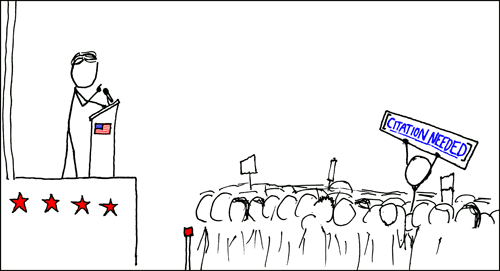
\includegraphics[width=1\textwidth]{Images/tirinha_randall_munroe.png}
    \caption{Tirinha de Randall Munroe que ilustra a página ``Wikipedia:Citation needed'', na Wikipédia anglófona com a seguinte legenda: ``A predefinição \{\{Carece de fontes\}\} visa promover discursos responsabilizáveis.'' \citewiki{enwiki_citation_needed}}
    \label{fig:tirinha_randall_munroe}
\end{figure}
\footnotetext{No original ``\textit{The \{\{Citation needed\}\} template aims to promote accountable discourse}''.}

Percebe-se então uma mudança crítica no trabalho do enciclopedista. Ao decidir se uma informação deve ter lugar em sua publicação, ele passa a ter sua atenção deslocada da preocupação com a ``veracidade'', para os conceitos complementares de ``verificabilidade'' e ``fiabilidade''.

Com isso, as principais discussões editoriais na Wikipédia são focadas na presença e na confiabilidade de fontes, e não diretamente na veracidade dos conteúdos individualizados. Ao contrário do que possa parecer a um primeiro olhar, este movimento não remove o especialista da cadeia de produção de conteúdo, mas apenas o desloca. Como explica Esteves (\citeyear[p.62]{esteves_as_2014}), ``\textit{Os especialistas continuam presentes, mas nas referências que devem fundamentar cada informação inserida nos artigos}". Assim, não é esperado que o especialista se apresente pessoalmente para os embates dentro da Wikipédia, mas que esse trabalho seja feito por porta-vozes seus. Um porta-voz, como bem sintetizado por Latour (\citeyear[p.108]{latour_ciencia_1987}),  ``\textit{é alguém que fala em lugar do que não fala. [...] um representante que expresse seus interesses, que fale em nome deles}''.

Dentro das disputas editoriais wikipédicas, os editores então terão maior chance de sucesso em seus argumentos e defesas de acordo com a reputação e o prestígio das vozes que estiver portando em seu discurso. Pois ``\textit{estar diante de um porta-voz não é o mesmo que estar diante de qualquer homem ou mulher comum. Não se está diante de Bill ou do Professor, mas diante de Bill, do Professor e mais as muitas coisas ou pessoas no interesse das quais eles estão falando}''. (\citep[p. 109]{latour_ciencia_1987}) Assim, ``\textit{longe de se livrar da autoridade do especialista, a Wikipédia depositou confiança nela}''\citep[p. 121]{jankowski_wikipedia_2013}.

É interessante notar que a participação dos porta-vozes não é algo que aconteça pela mera falta do especialista, e que tenderia a se diluir caso mais doutos se engajassem na escrita da enciclopédia colaborativa. A representação indireta através de porta-vozes é não só esperada como desejada pela comunidade, que entende esta terceirização como uma de suas inúmeras formas de garantir qualidade em sua produção editorial. Entende-se que o autor de uma pesquisa possa estar muito apegado a sua visão enviesada\footnote{No inglês ``\textit{biased}'', termo muito utilizado em debates no movimento Wikimedia sobre ``neutralidade''.} de um determinado assunto e tenda a apresentar conflito de interesses na escrita, pois se beneficiaria pessoal e diretamente de ter sua produção citada por um verbete da maior enciclopédia do mundo. \citewiki{ptwiki_conflito_interesses}

Seguindo esta linha de raciocínio, o editor não especialista, que atua traduzindo o conhecimento produzido por um autor (fonte primária) e já validado por uma entidade respeitada socialmente, sejam pares, jornalistas ou corpos editoriais (fonte secundária), terá maior traquejo para se movimentar entre diferentes abordagens de um mesmo tema, sendo a figura mais indicada para escrever um verbete enciclopédico de forma ``neutra''.\footnote{Ao longo do trabalho optamos por sempre escrever termos como ``neutro'' e ``neutralidade'' entre aspas para reforçar que são conceitos utilizados pela comunidade, mas não corroborados por este estudo.}

Esse movimento em busca de uma suposta ``neutralidade'' gera um curioso dualismo. Por um lado ele se sustenta necessariamente em uma crítica epistemológica à ciência moderna ocidental, que não teria em seus representantes o mero papel de reveladores de verdades naturais. Pois, é dito que se a eles fosse estimulado escrever diretamente os textos enciclopédicos relacionados a suas pesquisas, os verbetes acabariam maculados por interesses e política. Por outro lado, a busca por um texto enciclopédico neutro sugestiona que os wikipedistas, ao contrário dos cientistas, seriam sim capazes de escrever uma história de fatos e artefatos desprovida de subjetividades e enviesamentos.

``\textit{A contradição é flagrante e claramente sarcástica: de um lado, se todos podem editar, isto representaria naturalmente a diversidade de pontos de vista; de outro, espera-se que tudo isso se acalme num texto final de um único ponto de vista; no entanto, se todos podem editar sempre, não haveria texto final, mas em progresso incessante; nem se poderia imaginar que os textos, oriundos de incontáveis pontos vista, acabassem como peças sem ponto de vista (...) NPOV\footnote{Do inglês ``\textit{Neutral Point Of View}'', como é conhecida a política de neutralidade na Wikipédia.} aparece na cena como excrescência, um alinhamento a metodologias positivistas e que em nada funciona neste tipo de ambiente. É farsa cômoda.}'' \citep{demo_conhecimento_2009}

Mas, esse dualismo não parece ser uma grande questão para a maior parte da comunidade. A ``neutralidade'' em sua escrita é um dos pilares do Movimento Wikimedia \citewiki{ptwiki_cinco_pilares}, e usuários que tentam o questionar ou relativizar tender a ser rechaçados (a página "Wikipédia:Princípio da imparcialidade", que detalha a aplicação deste pilar, é linkada em mais de 250 mil outras páginas)\footnote{Dados disponiveis em https://xtools.wmflabs.org/articleinfo/pt.wikipedia.org/Wikipédia:Princípio\_da\_imparcialidade , acessado em 16 de junho de 2020.}. Ao mesmo tempo, é facilmente identificável no cotidiano da escrita wikipédica a utilização de fontes secundárias pouco conhecidas como referências para sustentação de afirmações, sem que seja realizado um escrutínio da suposta ``neutralidade'' de cada fonte. 

Assim, enquanto no discurso wikipédico da neutralidade pode ser facilmente identificada a presunção positivista enciclopédica da criação de um compêndio objetivo de todo o conhecimento humano \citep{esteves_as_2014}, o mesmo discurso não se apresenta tão estabilizado e inquestionável como o cientificismo positivista, e vê sua política editorial ser constantemente atacada por defensores do rigor científico. \citep{taraborelli_expert_2011} O protagonismo de não especialistas e a possibilidade de utilizar como fontes materiais produzidos por não cientistas coloca, para seus críticos, a Wikipédia em um local de produção de conteúdos não confiáveis.

Nos aproximamos assim de algo que pode ser visto como um paradoxo. A Wikipédia depõe a ciência do papel de um mero agente neutro revelador de verdades naturais. Mas, ao contrário do que poderíamos esperar, ao invés de com este movimento de destronamento da ciência, a comunidade buscar se sustentar em novas epistemologias não determinísticas de construção de verdades, a enciclopédia opta por se vender como o autêntico grande catalisador de verdades neutralizadas globais.

Essa curiosa situação paradoxal se propaga por todos os desdobramentos da defesa do modelo de produção colaborativa wiki e de sua suposta garantia de qualidade. Sua política explícita de utilização de fontes secundárias ``fiáveis'', simplesmente dá transparência à mesma dinâmica que estrutura o funcionamento de todas as ciências.

Seguindo esta linha de raciocínio, pode-se afirmar que essa transparência na construção de verdades acende um holofote sobre a fragilidade do argumento da existência de uma ``verdade una natural descoberta''. Com isso, para a Wikipédia ser ``verdadeira'' ou até mais confiável que outras enciclopédias, seria coerente que ela adotasse uma diferente visão da construção de fatos e artefatos diferente desta denunciada tradicional positivista.

Afinal, se é possível aos wikipedistas construírem uma verdade ``neutra'', como podem acusar os cientistas de não terem a mesma capacidade de criá-la e, ao mesmo tempo, utilizarem suas (dos cientistas) produções supostamente enviesadas como fontes de sustentação de sua (da Wikipédia) produção ``neutra''? 

\begin{figure}[H]
    \centering
    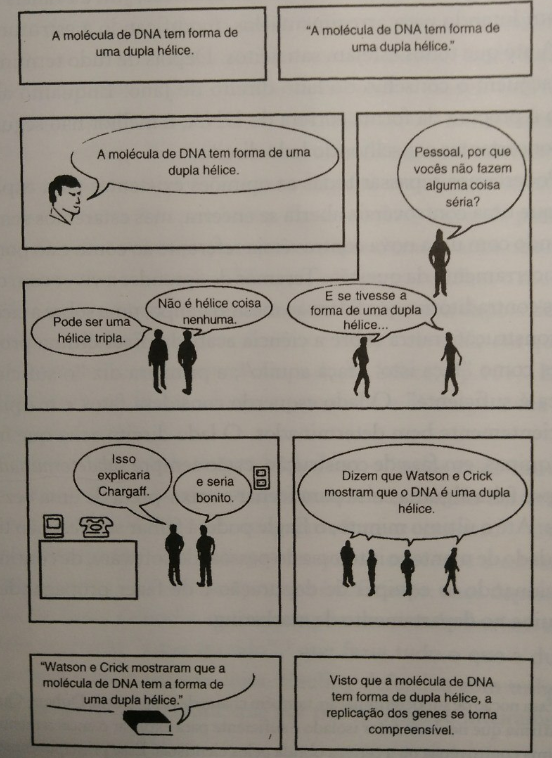
\includegraphics[width=0.5\textwidth]{Images/livro_ciencia_em_acao.png}
    \caption{Figura 1.6 do livro Ciência em Ação de Bruno Latour (\citeyear[p. 22]{latour_ciencia_1987}).}
    \label{fig:livro_ciencia_em_acao}
\end{figure}

Mas, mesmo perante esse aparente paradoxo, a escrita wikipédica apresenta algumas características que a diferenciam da escrita científica na estailibização de fatos. Na figura acima, retirada do livro Ciência em Ação de Bruno Latour, o último quadro onde ``\textit{vemos uma nova frase, sem aspas, escrita num livro}'' \citep[p.23]{latour_ciencia_1987} poderia muito bem ser a Wikipédia, só que desta vez a frase teria um pequeno número ao lado, indicando a referência que a sustenta. Em uma visão da ciência historicizada, como apresentada na figura, a transparência que a Wikipédia oferece ao leitor para saber onde dar o próximo passo, se desejar puxar o fio do novelo que levou à estabilização do fato ali apresentado, seria vista como um grande diferencial de qualidade se comparada com livros tradicionais que apresentam ``\textit{uma nova frase, sem aspas}'', como apontado por Latour.

``\textit{Inicialmente pelo menos, a Wikipédia tinha esta visão de seus textos: em progresso infindável, sem formato final, aberto à reconstrução de todos sem peias. Este estilo de 'fundamento sem fundo' (Demo, 2008) elabora uma expectativa dialética da produção de conhecimento que contrasta ostensivamente com outras inseridas na wikipedia de teor modernista e positivista, tal qual a noção de enciclopédia como guarda do conhecimento disponível, ou de neutralidade de sua produção pelos contribuintes, ou de verificabilidade dos conteúdos dos textos. A noção de conhecimento como dinâmica desconstrutiva/reconstrutiva é traída aí em nome de um estilo estabilizado, congelado e definitivo que já se poderia 'preservar'.}'' (\citeyear{demo_conhecimento_2009})

O discurso wikipedista de sempre dar transparência à procedência de suas afirmações é muito potente, e inclusive diversas vezes é apontado em palestras e apresentações como seu diferencial de qualidade perante outras produções. Porém, ao se apegar a citada ``\textit{expectativa dialética de teor modernista e positivista}'', a Wikipédia esvazia uma visão de mundo onde verdades não são reveladas, mas sim construídas, e se expõe mais fragilmente a críticas comumente vindas de setores ligados à academia e professores, que defendem com unhas e dentes que seus estudantes consultem livros (que seriam sempre confiáveis pois imutáveis) ao invés da Wikipédia (que não seria confiável pois ``qualquer um pode editar'').

Cabe aqui nos debruçarmos um pouco mais sobre o estranho duplipensar praticado por quem acusa a Wikipédia de não ser confiável mas ao mesmo tempo crê acriticamente em livros sem investigar a história de cada um individualmente. Qual seria afinal a garantia de qualidade de um livro impresso? A prensa teria por acaso algum compromisso moral com a verdade? Essa irônica pergunta nem sentido faz em nossa visão metodológica, pois já compreendemos que o processo de ``escrever verdades'' não é uma mera descrição de uma natureza revelada. Porém, apenas como exercício retórico, podemos brevemente assumir que essa visão naturalizada da construção de fatos e artefatos seja verdadeira. Assim, nossa pergunta deixa de ser mero despeito e ironia e se torna um questionamento relevante: como afinal impressoras mundo afora garantem que não estão sendo impressas mentiras? 

Perante a impossibilidade de encontrar uma resposta positiva para a pergunta, só nos resta concluir que a autoridade do livro é uma mera tradição/construção cultural/mercadológica, que aparenta não se sustentar nem mesmo no modelo conservador de verdades estanques reveladas, se feitas as perguntas certas. Aqui por honestidade intelectual, nos cabe observar que, como bem já disse algum antigo sábio português, ``pau que dá em Chico também dá em Francisco''. Ao desconstruirmos a autoridade emanada dos livros também estamos apontando o dedo para a Wikipédia. Pois afinal, esta utiliza os primeiros como fonte para seus textos. Por coerência metodológica, devemos então observar os efeitos de tal implicação para a escrita wikipédica. 

A grande diferença, inclusive autoproclamada como vantagem, do modelo de produção de conteúdo enciclopedista wiki para a tradicional escrita literária, está na intensa discussão sobre a fiabilidade de suas fontes. Livros \textit{per se} não são considerados fontes fiáveis pela Wikipédia. Para serem aceitos como dignos de credibilidade, não basta palavras terem sido convertidas em tinta bem recebida pelo papel. Seus autores e corpos editoriais precisam ter reputações e reconhecimentos que sejam entendidos como relevantes pela comunidade, para então serem acreditados como fontes fiáveis.

Seguindo o fio desta reflexão, é quase inevitável encontrar a curiosa conclusão de que a principal crítica feita à qualidade da Wikipédia (de que qualquer um pode editar), se apontada para o modelo dito tradicional de produção de conhecimento (o mesmo exaltado pelos críticos da metodologia wiki), revelará uma enorme probabilidade de ``mentiras'' serem propagadas através de livros, revistas, apostilas e manuais. Pois, afinal, hoje em dia ``qualquer um pode editar um livro''.

Enquanto isso, ironicamente, o modelo wiki apresenta regras que se preocupam em mitigar esse risco, oferecendo ao hesitante leitor formas razoavelmente transparentes de rastrear a validação feita por terceiros das informações ali apresentadas, propiciando assim maior enredamento e, por consequência, robustez aos textos ali publicados.